\documentclass{presentation}

% some details about the cover page
\title[slide $\text{\insertframenumber}$]{Efficient Algorithm}
\subtitle{Jump points}
\author{Rademacher, Loka}
\date{\today}
\institute{
    Department of Computer Science \\
    University of Bonn
}

\begin{document}



\begin{frame}
    \titlepage
\end{frame}

\begin{frame}{Inhalt}
    \begin{itemize}
        \item Rucksackproblem
        \item Core-Algorithmus
        \item Bestimmung des Teilungsobjekts
        \item Nemhauser-Ullmann Algorithmus
        \item Experimentelle Analyse
    \end{itemize}
\end{frame}



\begin{frame}
    \bigbox{Rucksackproblem}
\end{frame}



\begin{frame}
    \frametitle{Rucksackproblem}
    \begin{itemize}
        \item Einen Rucksack mit beschränkter Größe
        \item Eine Menge vom Objekten, die eingepackt werden sollen
        \item Jedes Objekt hat einen Nutzen und ein Gewicht
        \pause

        \item Wie packt man den Rucksack am besten?
        \item Problem ist $\mathrm{NP}$-vollständig
    \end{itemize}
\end{frame}



\begin{frame}
    \frametitle{Formale Definitionen}
    \begin{eqnarray*}
        \text{maximiere} & & p^T x = \sum_{i=1}^n p_i x_i \\
        \text{unter} & & w^T x = \sum_{i=1}^n w_i x_i \leq W \\
        \text{mit} & & x \in \{0,1\}^n
    \end{eqnarray*}
    \pause

    Das fraktionales Rucksackproblem erlaubt $x \in [0,1]^n$.
\end{frame}



\begin{frame}
    \bigbox{Core-Algorithmus}
\end{frame}



\begin{frame}
    \frametitle{Idee}
    \begin{itemize}
        \item Fraktionales Rucksackproblem lösen
        \item Objekte austauschen um die ganzzahlige Lösung zu finden
        \item Tauschkandidaten sind nur wenige Objekte
        \item Menge der Kandidaten heißt Core
    \end{itemize}
\end{frame}



\begin{frame}
    \frametitle{Umsetzung}
    \begin{itemize}
        \item Objekte in drei Mengen einteilen
        \begin{itemize}
            \item Core - Tauschkandidaten
            \item Objekte, welche zur Lösung gehören
            \item Objekte, welche nicht zur Lösung gehören
        \end{itemize}
        \pause

        \item Core und Restgewicht ergeben neue Probleminstanz % $\mathrm{KP}$-Instanz
        \item Instanz kann mit beliebigem Algorithmus gelöst werden
    \end{itemize}
\end{frame}

\begin{frame}
    \frametitle{Definition des Core}
    
    \begin{itemize}
        \item Sei $\bar{x}$ die Loesung des fraktionalen Rucksackproblems
        \pause
        
        \item Struktur ist $(1, 1, ..., 1, f, 0, 0, ..., 0)$ mit $f > 0$
        \pause
        
        \item Das Objekt $k$ mit Gewichtung $f$ heißt Teilungsobjekt und hat eine Effizienz $r$
        \pause
        
        \item Der Verlust eines Objekts ist definiert mit $l_i = |p_i - r \cdot w_i|$
    \end{itemize}
\end{frame}

\begin{frame}
    \frametitle{Definition des Core}
    \begin{itemize}
        \item Es gilt $\Gamma := p^T \bar{x} - p^T x^{\star} = r (W - w^T x^{\star}) + \sum_{i \in \Delta(x^{\star})} l_i$
        \pause

        \item Ein Objekt, welches einen Verlust $l_i > \Gamma$ hat, gehört nicht zum Core
        \pause

        \item $\Gamma$ kann abgeschätzt werden, indem statt der optimalen Lösungen eine beliebige ganzzahlige Lösung verwendet wird
        \pause

        \item Je besser die ganzzahlige Lösung, desto besser die Abschätzung
    \end{itemize}
\end{frame}



\begin{frame}
    \frametitle{Pseudocode}
    \textsc{\large ExpandingCore}
    \begin{algorithmic}[1]

        \State Berechne die optimale fraktionale Lösung $\bar{x}$
        \State $\gamma \gets p_k \bar{x}_k$
        \pause

        \Repeat
            \State $i \gets$ Index eines Objekts mit minimalem Verlust
            \State Erweitere Core um Objekt $i$
            \State $x \gets$ nutzengrößte gültige Lösung aus dem Core
            \State $\gamma \gets p^T \bar{x} - p^T x$
        \Until {$l_i \geq \gamma$}
        \pause

        \State \Return x

    \end{algorithmic}

    Erwartete Laufzeit liegt in $\mathcal{O}(n\:polylog(n))$.
\end{frame}



\begin{frame}
    \bigbox{Bestimmung des Teilungsobjekts}
\end{frame}



\begin{frame}
    \frametitle{Greedy-Algorithmus}
    \begin{itemize}
        \item Sortieren der Objekte nach Effizienz
        \pause

        \item Solange noch Kapazität über ist, Objekt mit höchster Effizienz einpacken
        \pause

        \item Rucksack mit nächstem Objekt voll machen
    \end{itemize}
\end{frame}



\begin{frame}
    \frametitle{Linearzeit-Algorithmus}
    \begin{itemize}
        \item Verzichten auf vorheriges Sortieren
        \pause

        \item Algorithmus ähnlich zu \textsc{Quickselect}
        \begin{itemize}
            \item k. kleinstes Element finden ohne zu sortieren
        \end{itemize}
        \pause

        \item Rekursiver Algorithmus mit Partitionierung (hier \textsc{Hoare-Partition})
    \end{itemize}
\end{frame}



\begin{frame}
    \frametitle{Aufteilung der Partitionen}
    \begin{figure}[!htb]
        \centering
        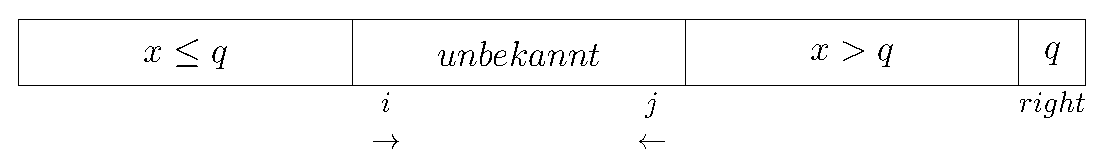
\includegraphics[scale=.5]{res/partition1.eps}
        \caption{\textsc{Partition} mit einem Pivot}
        \label{fig:partition1}
    \end{figure}
\end{frame}



\begin{frame}
    \frametitle{Wahl der Pivots}
    \begin{itemize}
        \item Feste Wahl
        \pause

        \item Zufällige Wahl
        \pause

        \item Median einer Teilmenge
        \begin{itemize}
            \item Feste Größe (\textsc{Median of Three})
            \item Größe abhängig von Arraylänge $n$ (z.B. $\sqrt{n}$)
        \end{itemize}
        \pause

        \item Median in Linearzeit bestimmen
    \end{itemize}
\end{frame}



\begin{frame}[fragile]
    \frametitle{Pseudocode}
    \textsc{\large BreakitemB}
    \begin{algorithmic}[1]
        \If {$left > right$}
            \State $q \gets $ \Call{Partition}{$A$, $left$, $right$}
            \State $Wq \gets \sum_{i=left}^{q} w_i$
            \pause

            \If {$Wq > t$}
                \State \Return \Call{BreakitemB}{$A$, $left$, $q-1$, $t$}
            \pause
            \Else
                \State \Return $(q-left+1)$ + \Call{BreakitemB}{$A$, $q+1$, $right$, $t-Wq$}
            \EndIf
        \EndIf
        \pause

        \State \Return 0
    \end{algorithmic}
\end{frame}



\begin{frame}
    \frametitle{DualPivotQuicksort}
    \begin{itemize}
        \item 2009 wurde eine verbesserte Version von \textsc{Quicksort} veröffentlicht
        \item Schnellester Sortieralgorithmus, Java 7 Standard
        \item Partitioniert mit zwei statt einem Pivotelement
        \item Verbesserungen auf \textsc{BreakitemB} übertragen
        \item Laufzeit unterscheidet sich nur um eine Konstante
    \end{itemize}
\end{frame}



\begin{frame}
    \frametitle{Aufteilung der Partitionen}
    \begin{figure}[!htb]
        \centering
        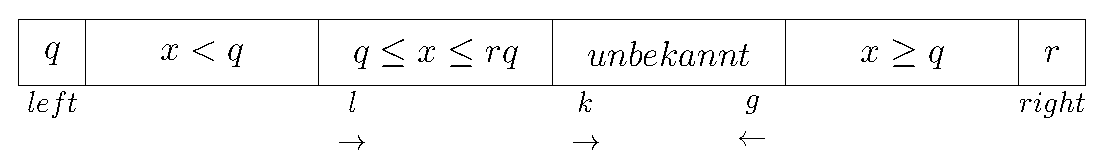
\includegraphics[scale=.5]{res/partition2.eps}
        \caption{\textsc{Partition} mit zwei Pivots}
        \label{fig:partition2}
    \end{figure}
\end{frame}



\begin{frame}
    \frametitle{Experimentelle Analyse}
    \begin{figure}[!htb]
        \centering
        \includegraphics[scale=0.4]{res/breakitem_time_average.png}
        \caption{durchschnittliche Laufzeiten der \textsc{Breakitem} Algorithmen}
        \label{fig:breakitem_time_average}
    \end{figure}
\end{frame}



\begin{frame}
    \bigbox{Nemhauser-Ullmann Algorithmus}
\end{frame}



% \begin{frame}
%     \frametitle{Lösungsvektor x}
%     \begin{itemize}
%         \item $x \in \{0, 1\}^n$ heißt Lösungsvektor
%         \pause
%
%         \item $x$ heißt zulässig $:\iff w^T x \leq W$
%         \pause
%
%         \item $x$ enthält das i. Objekt $:\iff x_i = 1$
%         \pause
%
%         \item $x$ heißt Pareto-optimal $:\iff \nexists y \in \{0, 1\}^n: p^T x \leq p^T y \land w^T x \geq w^T y$\\ (eine Ungleichung ist streng)
%     \end{itemize}
% \end{frame}



\begin{frame}
    \frametitle{Idee}
    \begin{itemize}
        \item $x$ ist pareto-optimal $\iff \nexists y \in \{0, 1\}^n: p^T x \leq p^T y \land w^T x \geq w^T y$
        (eine Ungleichung ist streng)
        \pause

        \item $\mathcal{P}_i$ ist die Menge aller pareto optimalen Lösungsvektoren, die nur die ersten i Elemente enthalten
        \pause

        \item $\mathcal{P}_i$ induktiv berechnen
        \pause

        \item $\mathcal{P}_i = \{ x \mid x \in \mathcal{P}_{i-1} \cup \mathcal{P}_{i-1}^{+i} \: \land x\text{ pareto-optimal}\}$
    \end{itemize}
\end{frame}



% \begin{frame}
%     \frametitle{Idee}
%
%     optimaler Lösungsvektor für KP ist $\in \mathcal{P}_n$\\
%     Beweis:\\
%     Annahme: es gibt y optimal $\in \{0, 1\}^n \setminus \mathcal{P}_n$.\\
%     Dann gilt $\nexists x \in \mathcal{P}_n: w^T x \leq w^T y \land p^T x > p^T y$.\\
%     Daraus folgt y ist pareto-optimal.\\
%     Das ist ein Widerspruch zu $y \notin \mathcal{P}_n$.
% \end{frame}



\begin{frame}[fragile]
    \frametitle{Pseudocode}
    \textsc{\large Nemhauser-Ullmann Algorithmus}
    \begin{algorithmic}[1]
        \State $\mathcal{P}_0  \gets \{ 0^n \}$
        \pause

        \For{i = 1, 2, ..., n}
            \State $\mathcal{Q}_i \gets \mathcal{P}_{i-1} \cup \mathcal{P}_{i-1}^{+i}$
            \State $\mathcal{P}_i \gets \{x \in \mathcal{Q}_i \mid \nexists y \in \mathcal{Q}_i: y$ dominiert $x \}$
        \EndFor
        \pause

        \State \Return $x^\star \gets$ arg max$_{x \in \mathcal{P}_n}\{p^T x \mid w^T x \leq W \}$
    \end{algorithmic}

\end{frame}



% \begin{frame}
%     \frametitle{Korrektheit}
%     \begin{itemize}
%         \item optimale Lösung $\in \mathcal{P}_n$
%         \item Algorithmus liefert die gewünschte Menge
%     \end{itemize}
% \end{frame}



\begin{frame}
    \frametitle{Laufzeit}
    $$\mathcal O(\sum_{i=0}^{n-1} |\mathcal{P}_i|)$$
    \pause
    $$ = \mathcal O(\sum_{i=0}^{n-1} |\mathcal{P}_n|)$$
    $$ = \mathcal O(n \cdot |\mathcal{P}_n|)$$
    $$ = \mathcal O(n \cdot \phi n^2)$$
    % $$ = \mathcal O(\phi n^3)$$
\end{frame}



\begin{frame}
    \bigbox{Experimentelle Analyse}
\end{frame}



\begin{frame}
    \frametitle{Testumgebung}
    \begin{itemize}
        \item Nutzen und Gewichte sind uniform zufällig gewählt
        \pause

        \item Kapazität wird durch $\beta \cdot \sum_{i=1}^n w_i$ bestimmt, $\beta \in [0, 1]$
        \pause

        \item 1000 Wiederholung pro Testpunkt bei \textsc{ExpandingCore}
        \pause

        \item Je nach Graph wird der Durchschnitt oder die Varianz abgebildet
    \end{itemize}
\end{frame}



\begin{frame}
    \frametitle{Experimentelle Analyse}
    \begin{figure}[!htb]
        \centering
        \includegraphics[scale=0.4]{res/core_time_average.png}
        \caption{durchschnittliche Laufzeit von \textsc{ExpandingCore}}
        \label{fig:core_time_average}
    \end{figure}
\end{frame}



\begin{frame}
    \frametitle{Experimentelle Analyse}
    \begin{figure}[!htb]
        \centering
        \includegraphics[scale=0.4]{res/core_time.png}
        \caption{Laufzeit von \textsc{ExpandingCore} als Boxplot}
        \label{fig:core_time}
    \end{figure}
\end{frame}



\begin{frame}
    \frametitle{Experimentelle Analyse}
    \begin{figure}[!htb]
        \centering
        \includegraphics[scale=0.4]{res/core_size.png}
        \caption{Größe des Core}
        \label{fig:core_size}
    \end{figure}
\end{frame}



\begin{frame}
    \frametitle{Experimentelle Analyse}
    \begin{figure}[!htb]
        \centering
        \includegraphics[scale=0.4]{res/core_final_pp.png}
        \caption{Maximum aller gespeicherten Paretopunkte}
        \label{fig:core_final_pp}
    \end{figure}
\end{frame}



\begin{frame}
    \frametitle{Experimentelle Analyse}
    \begin{figure}[!htb]
        \centering
        \includegraphics[scale=0.4]{res/core_total_pp.png}
        \caption{Summe aller gespeicherten Paretopunkte}
        \label{fig:core_total_pp}
    \end{figure}
\end{frame}



\begin{frame}
    \frametitle{Quellen}
    \begin{itemize}
        \item Vortrag basiert auf meiner Bachelorarbeit \textit{Experimentelle Analyse von Core-Algorithmen zur Lösung des Rucksackproblems}
        \item Alle Abbildungen sind dieser entnommen
    \end{itemize}
\end{frame}



\begin{frame}
    \bigbox{Vielen Dank für Ihre Aufmerksamkeit!}
\end{frame}

\end{document}
